\section{Problem\'atica}

El desarrollo de un sistema de punto de venta para \textit{Wallpa Wawqi} surgi\'o de la necesidad de centralizar el registro, la administraci\'on y la consulta de la informaci\'on del negocio en una sola plataforma. Antes de este proyecto, la gesti\'on de productos, sesiones de empleados y actualizaci\'on del inventario depend\'ia de procesos manuales que pod\'ian generar demoras, errores de captura y una disponibilidad limitada de la informaci\'on en tiempo real.

Adem\'as, el negocio requer\'ia una soluci\'on accesible desde la web, capaz de almacenar datos de forma persistente y permitir operaciones de creaci\'on, lectura, actualizaci\'on y eliminaci\'on sobre los productos. Tambi\'en se necesitaba una interfaz clara para el usuario final, con una estructura que facilitara el uso cotidiano sin sacrificar orden ni estabilidad en la gesti\'on interna.

Otro aspecto importante fue la necesidad de separar responsabilidades dentro del sistema. Si la l\'ogica de negocio, la persistencia y la presentaci\'on se manten\'ian mezcladas, el mantenimiento posterior del proyecto resultar\'ia m\'as complejo. Por ello, desde el inicio se plante\'o una arquitectura modular que permitiera identificar con claridad las funciones de cada componente.

\begin{figure}[H]
\centering
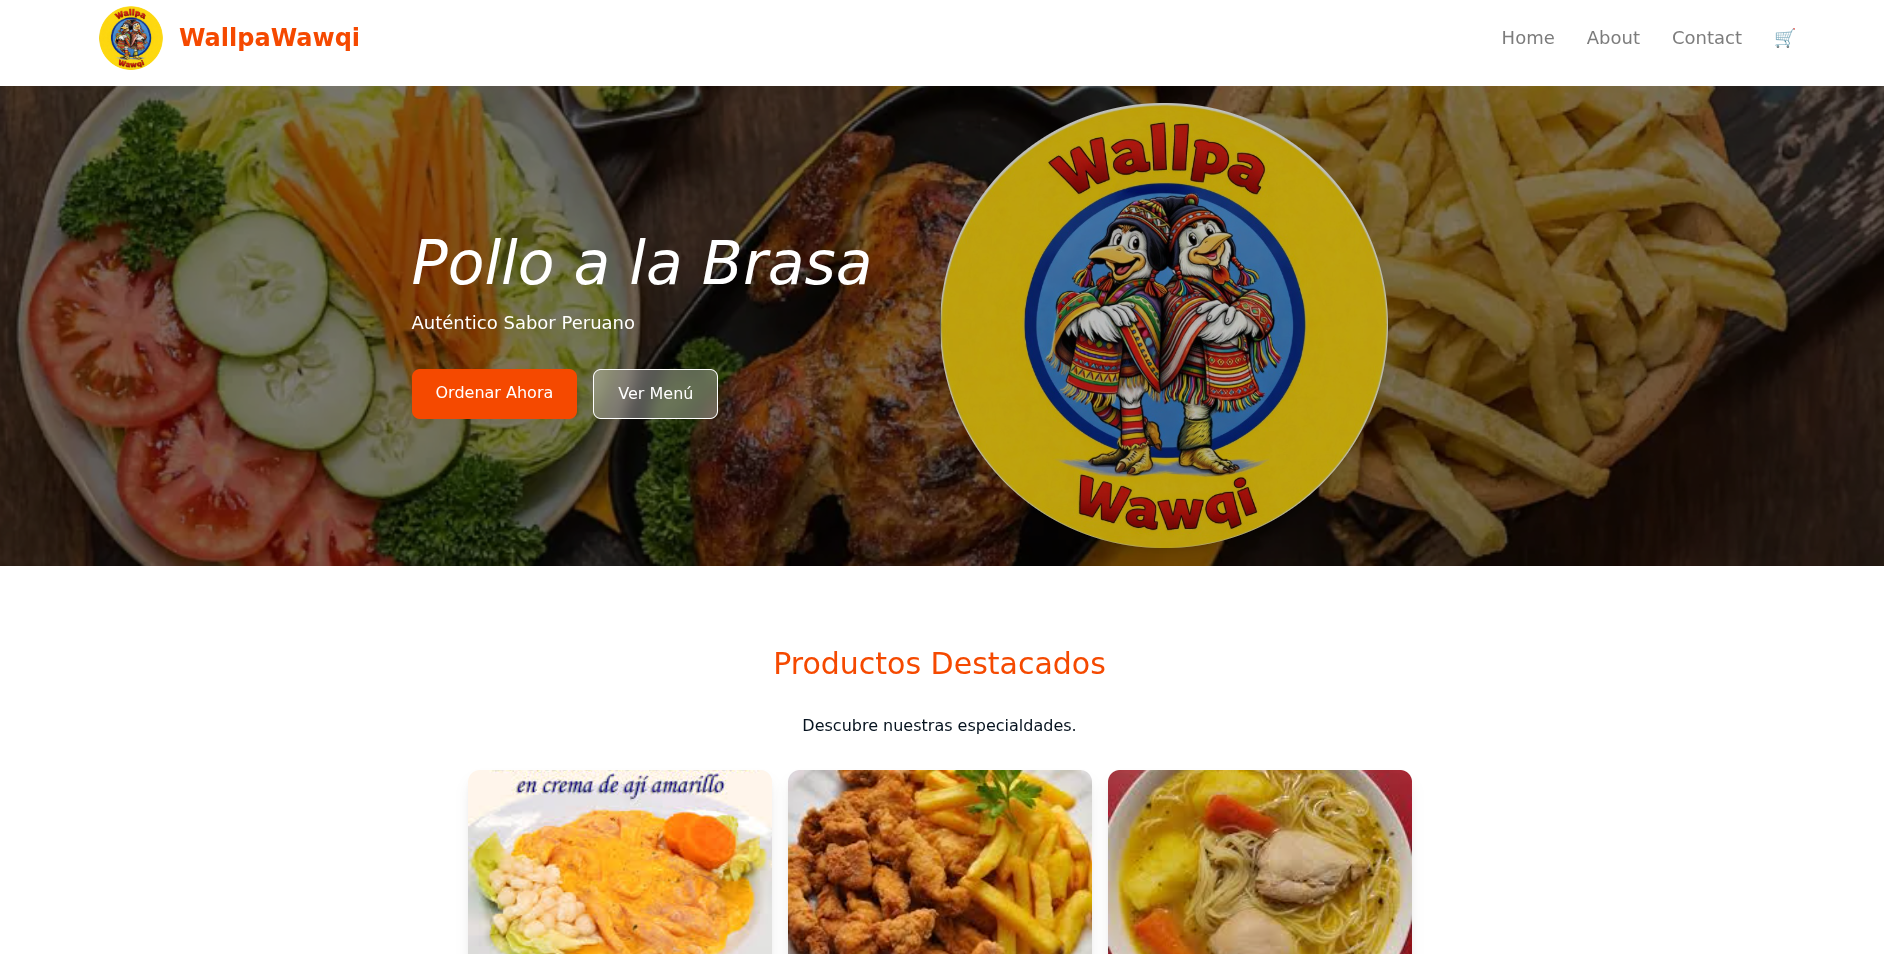
\includegraphics[width=0.86\textwidth]{assets/capturas/image.png}
\caption{Referencia visual de la situaci\'on inicial del sistema. Se observa como no hay un sistema de login, orden de compra o registro de pruducto.}
\label{fig:problematicavisual}
\end{figure}

\section{Soluci\'on}

Para responder a esta problem\'atica se implement\'o una arquitectura dividida en backend y frontend. El backend fue desarrollado en Java, utilizando una estructura por capas con clases de dominio, acceso a datos y servicios auxiliares. En \texttt{ProductoDAO} y \texttt{EmpleadoDAO} se centraliza el acceso a la base de datos PostgreSQL, mientras que \texttt{DatabaseConnection} gestiona la conexi\'on con el motor de datos y \texttt{CloudinaryService} se encarga de almacenar las im\'agenes de los productos en la nube.

La aplicaci\'on expone servicios HTTP mediante \texttt{HttpServer} para las operaciones de autenticaci\'on, consulta, creaci\'on, actualizaci\'on y eliminaci\'on de productos. Adem\'as, se integraron clases como \texttt{EmpleadoSesion}, \texttt{Categoria}, \texttt{Inventario} y las subclases de personal para representar de forma m\'as clara la estructura del negocio. Esto permite que cada entidad mantenga una responsabilidad concreta dentro del sistema.

Por su parte, el frontend fue construido con Astro y desplegado en Vercel, ofreciendo una interfaz moderna para visualizaci\'on de productos, registro, edici\'on y pedidos. Esta separaci\'on permite que el backend se ejecute en Railway y que la base de datos PostgreSQL se mantenga en Render.com, logrando una distribuci\'on adecuada de servicios y una mejor organizaci\'on del proyecto.

\begin{figure}[H]
\centering
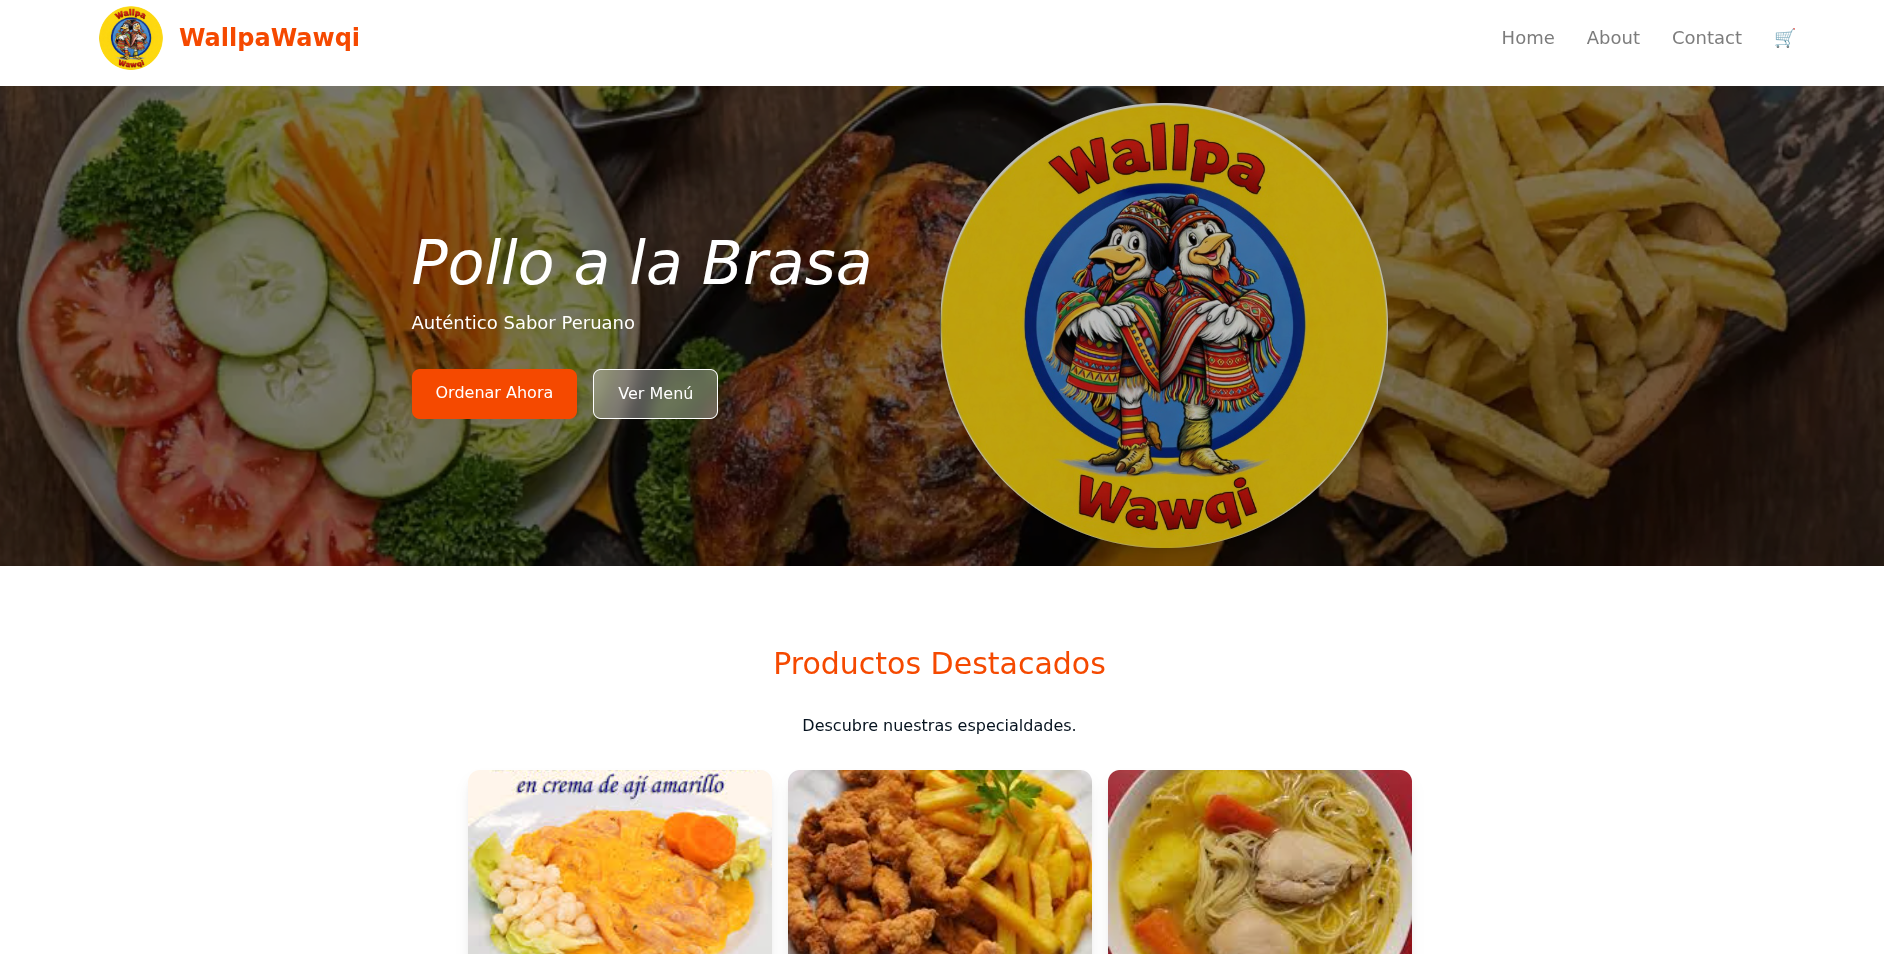
\includegraphics[width=0.86\textwidth]{assets/capturas/image2.png}
\caption{Vista principal del frontend del sistema.}
\label{fig:frontendprincipal}
\end{figure}

\begin{figure}[H]
\centering
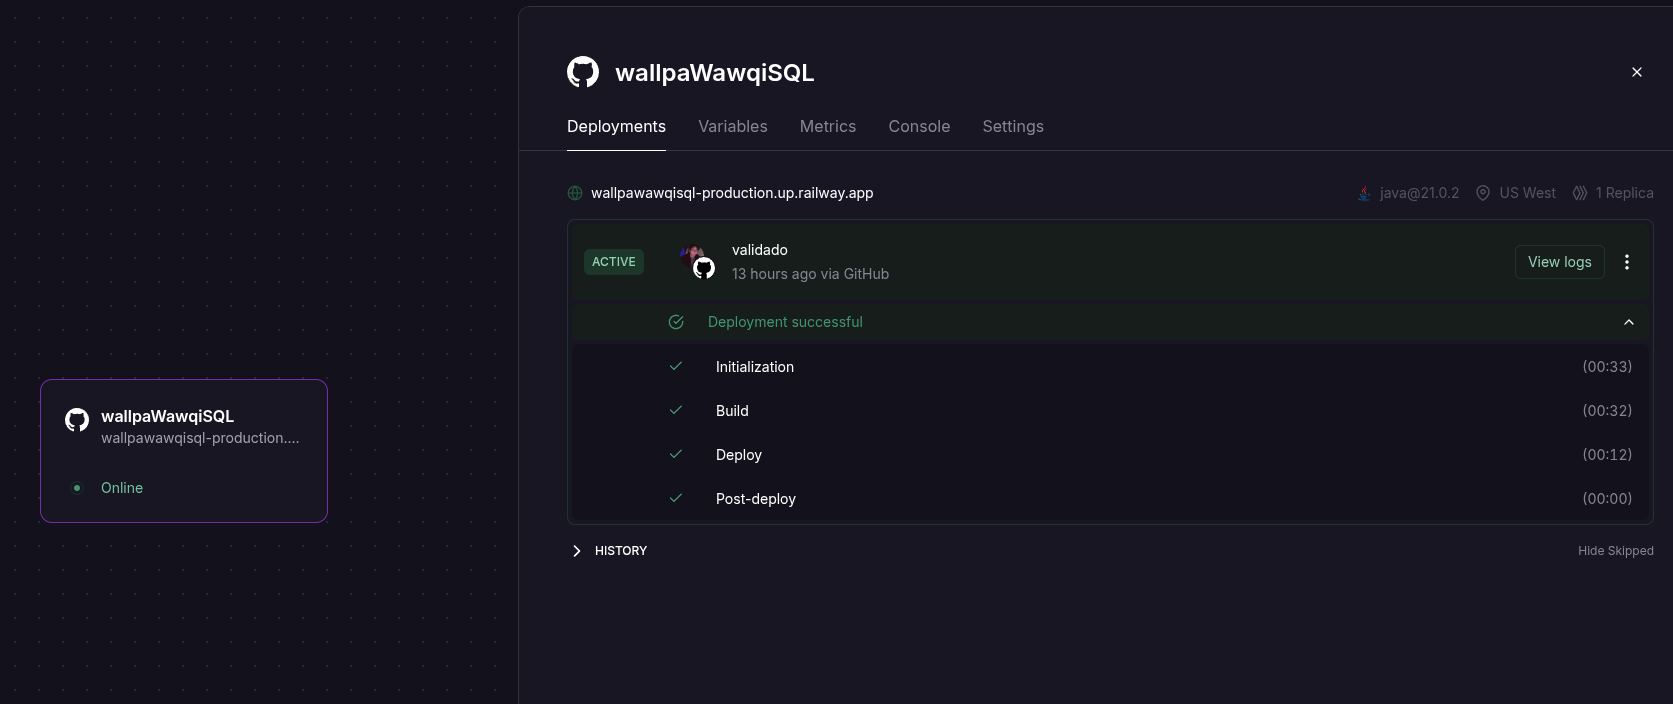
\includegraphics[width=0.86\textwidth]{assets/capturas/image3.png}
\caption{Referencia visual del backend en funcionamiento.}
\label{fig:backendprincipal}
\end{figure}

\section{Conclusiones}

El proyecto permiti\'o consolidar una soluci\'on funcional que integra persistencia de datos, servicios web y una interfaz web responsiva para la gesti\'on de un sistema de punto de venta. La distribuci\'on entre backend, frontend y base de datos facilit\'o una implementaci\'on ordenada, manteniendo cada tecnolog\'ia enfocada en una funci\'on espec\'ifica dentro del sistema.

Asimismo, el uso de PostgreSQL, Railway, Vercel y Render.com demuestra que es posible desplegar una aplicaci\'on completa con componentes desacoplados y accesibles desde la web. En t\'erminos acad\'emicos, el proyecto puso en pr\'actica principios de programaci\'on orientada a objetos, comunicaci\'on cliente-servidor y organizaci\'on modular del software.

El trabajo tambi\'en evidenci\'o la importancia de definir desde el inicio una estructura clara para los modelos, los servicios y el acceso a datos. Esa decisi\'on facilit\'o el desarrollo posterior y permiti\'o mantener una base t\'ecnica comprensible para futuras mejoras.

\section{Recomendaciones}

Se recomienda ampliar el sistema incorporando autenticaci\'on m\'as robusta, validaciones adicionales en el frontend y control de errores m\'as detallado en el backend para mejorar la seguridad y la experiencia de uso. Tambi\'en ser\'ia conveniente agregar reportes de ventas, categor\'ias din\'amicas, historial de operaciones y roles de usuario con permisos diferenciados.

De igual forma, se sugiere optimizar la interfaz para dispositivos m\'oviles y mantener una documentaci\'on t\'ecnica actualizada de la arquitectura desplegada. Las muestras, capturas de pantalla y demostraciones del funcionamiento del sistema se realizar\'an durante la exposici\'on para evidenciar el alcance real de la soluci\'on implementada.

Finalmente, se recomienda conservar los espacios reservados para figuras hasta contar con las capturas definitivas, de modo que el documento final mantenga coherencia visual y respete la estructura prevista para la presentaci\'on.
